\documentclass[10pt]{beamer}
\usepackage{fancybox}
%\usepackage{media9}
\usepackage{multimedia}
\usepackage{animate}
\usepackage{amssymb,amsmath}
\usepackage{tikz}

\let\Tiny\tiny% http://tex.stackexchange.com/q/58087/5764
\definecolor{BlueViolet}{RGB}{199,21,133}
\definecolor{KakiGreen}{RGB}{50,205,50}
\definecolor{DarkOrange}{RGB}{235,135,0}

\usetheme{lunchmeeting}
\graphicspath{{pics/}}

\newcommand{\sub}[1]{_{\text{#1}}}
\newcommand{\shadowfig}[2]{\tikz\node[drop shadow={shadow scale=0.95, top color=gray, opacity=0.5}]{\fcolorbox{white}{white}{\includegraphics[scale=#2]{#1}}};}
\newcommand\Wider[2][3em]{%
\makebox[\linewidth][c]{%
  \begin{minipage}{\dimexpr\textwidth+#1\relax}
  \raggedright#2
  \end{minipage}%
  }%
}
% -- Command for adding references in the footline
\newcommand{\footlineextra}[1]{
    \begin{tikzpicture}[remember picture,overlay]
        \node[yshift=2ex,anchor=south west] at (current page.south west) {\usebeamerfont{author in head/foot}\hspace{2ex}\Tiny{#1}};
    \end{tikzpicture}
}

\setbeamercolor{normal text}{fg=darkgray,bg=}
\setbeamercolor{alerted text}{fg=DarkOrange,bg=}
\usebeamercolor{normal text}
\setbeamersize{text margin left=5mm,text margin right=10mm}

\title{Understanding and controlling coverage biases in single-cell WGBS-seq}
\date{16/04/2018}
\author{Emma Dann, Master internship}


\includeonlyframes{current}
\begin{document}

% Title slide
\begin{frame}
 \titlepage
\end{frame}



\begin{frame}{Uneven coverage in scBS-seq data}
  \begin{figure}
    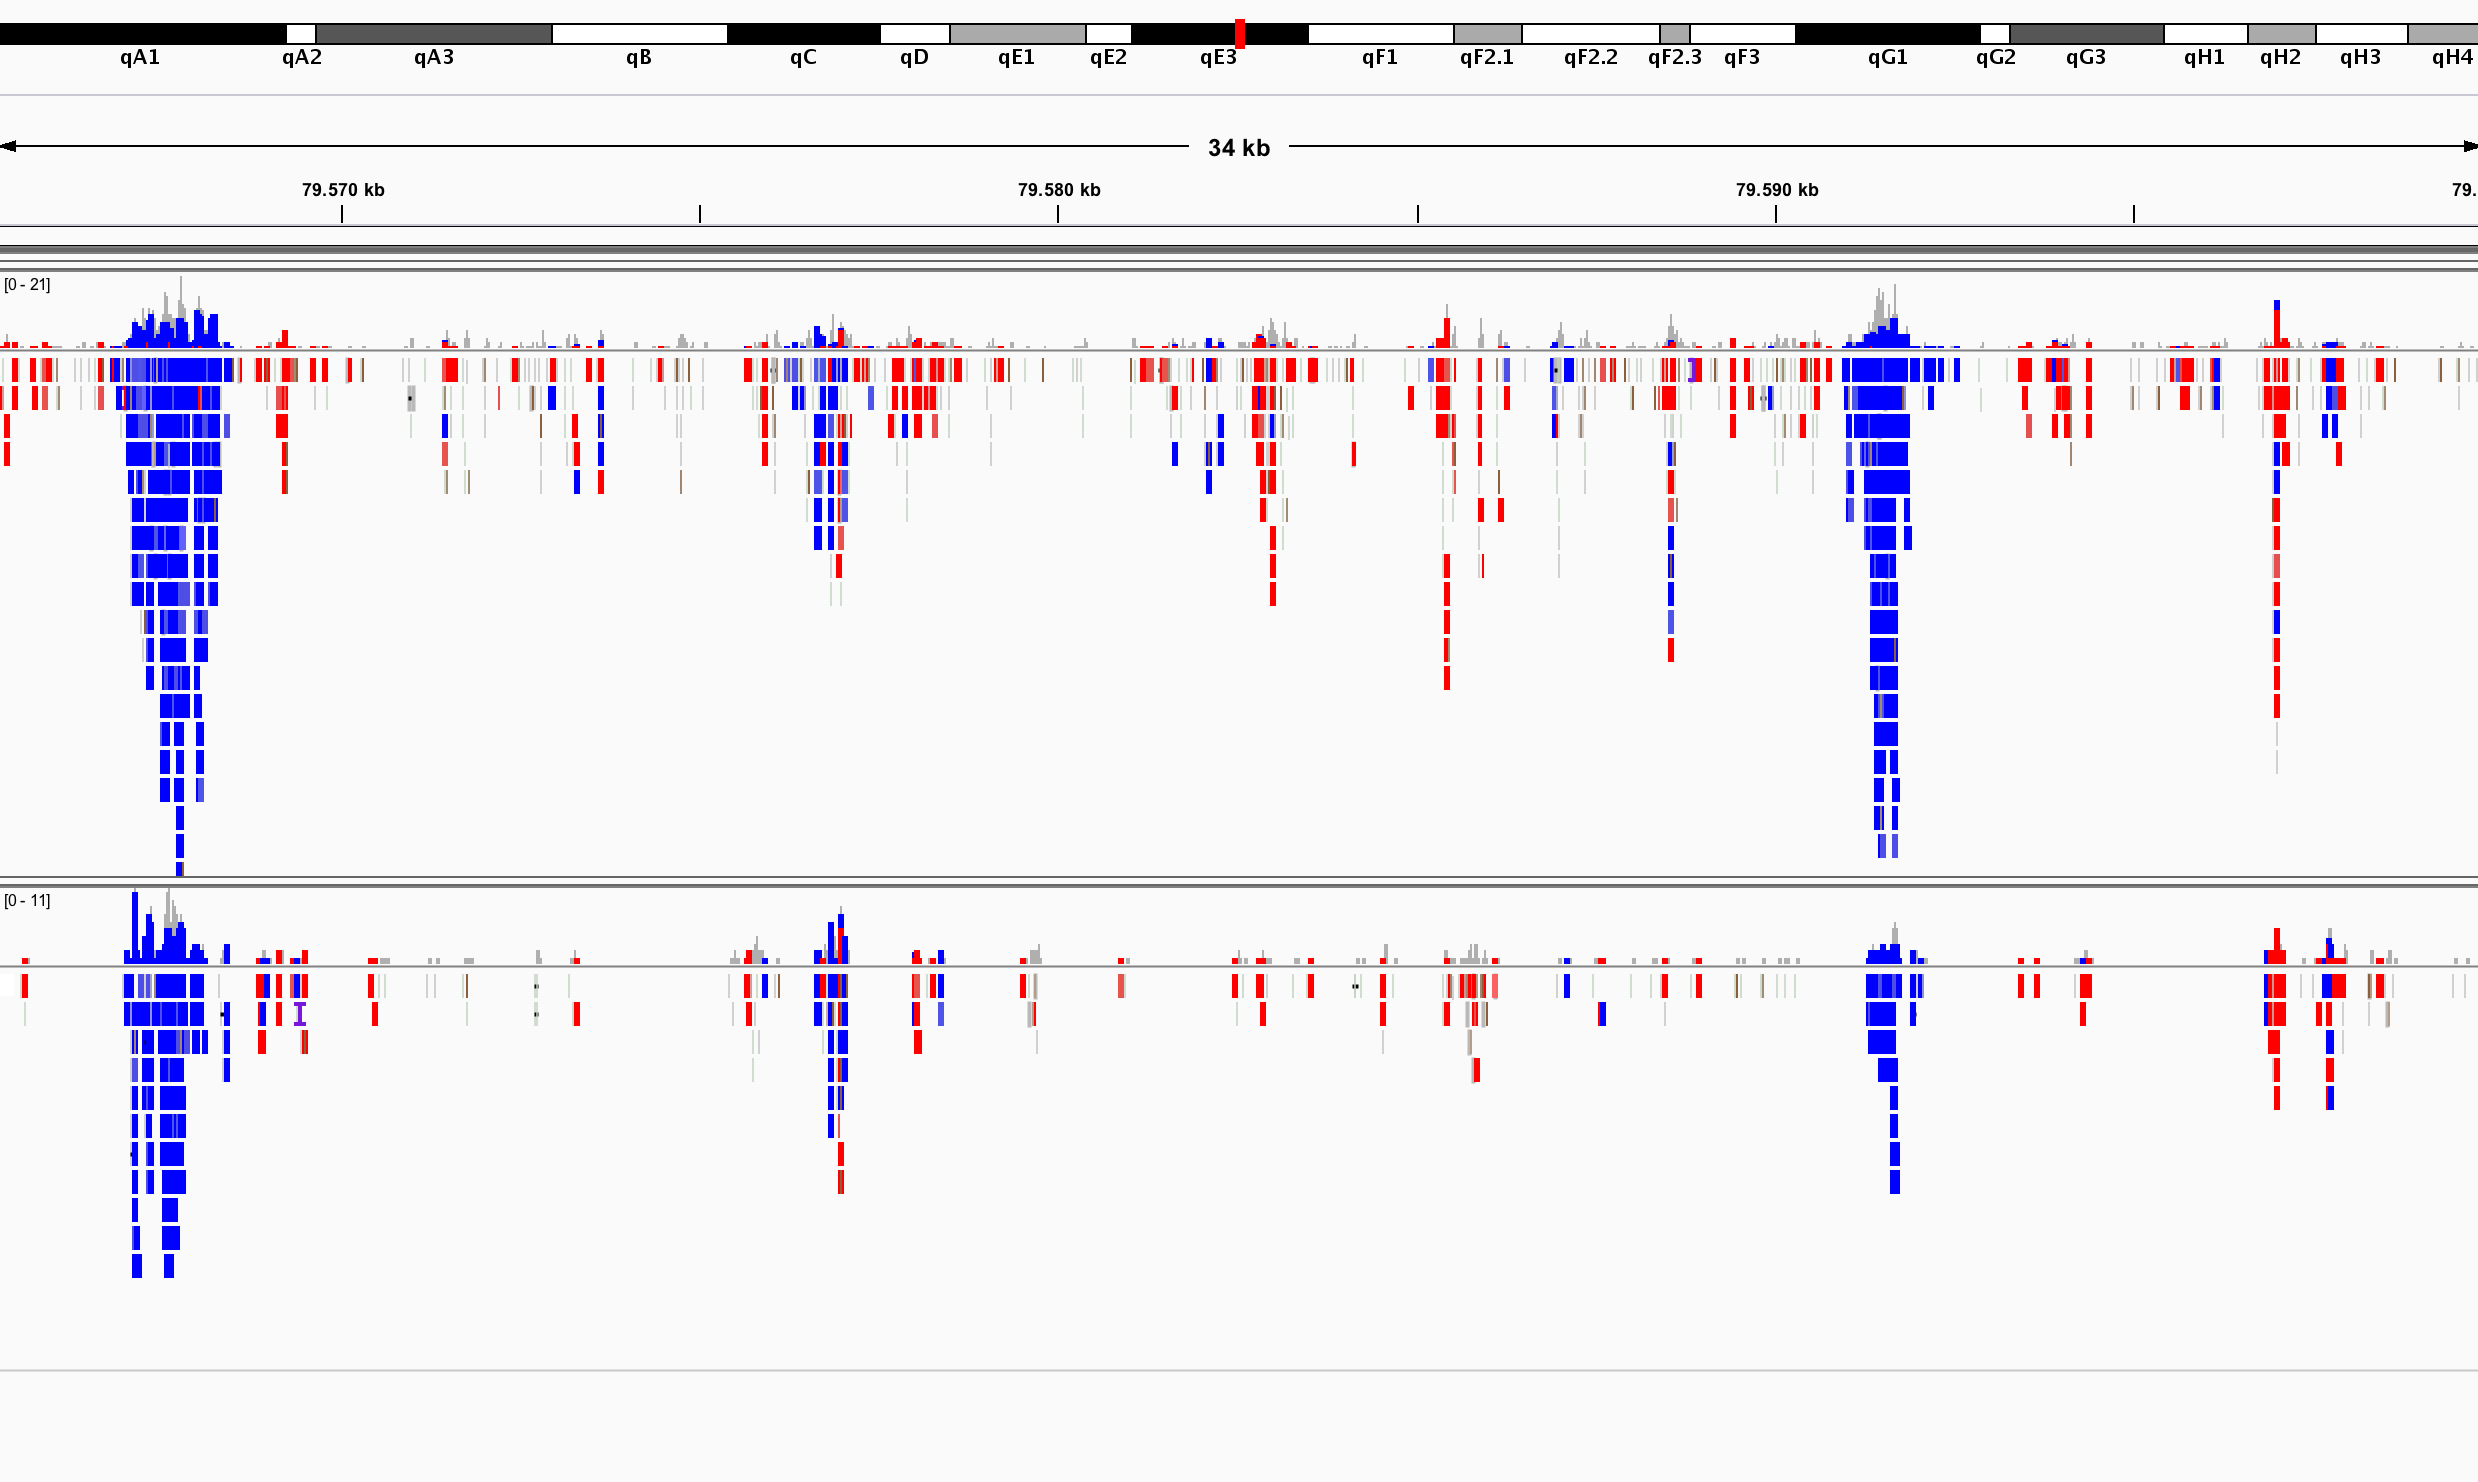
\includegraphics[scale=0.25, trim={0 0 0 16cm}, clip]{purifiedDNA.png}
  \end{figure}
  Mouse intestine, 100 cells
\end{frame}


\begin{frame}{Uneven coverage in scBS-seq data}
  \vspace{-0.2cm}
  \begin{figure}
      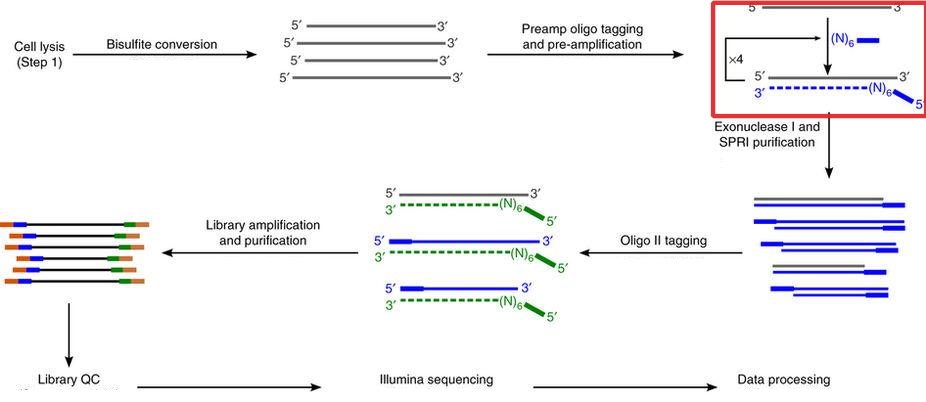
\includegraphics[scale=0.23]{wolf_reik_prot_preamp.png}
  \end{figure}
  \footlineextra{Clark et al. Nature Protocols 2017}
  \begin{figure}
      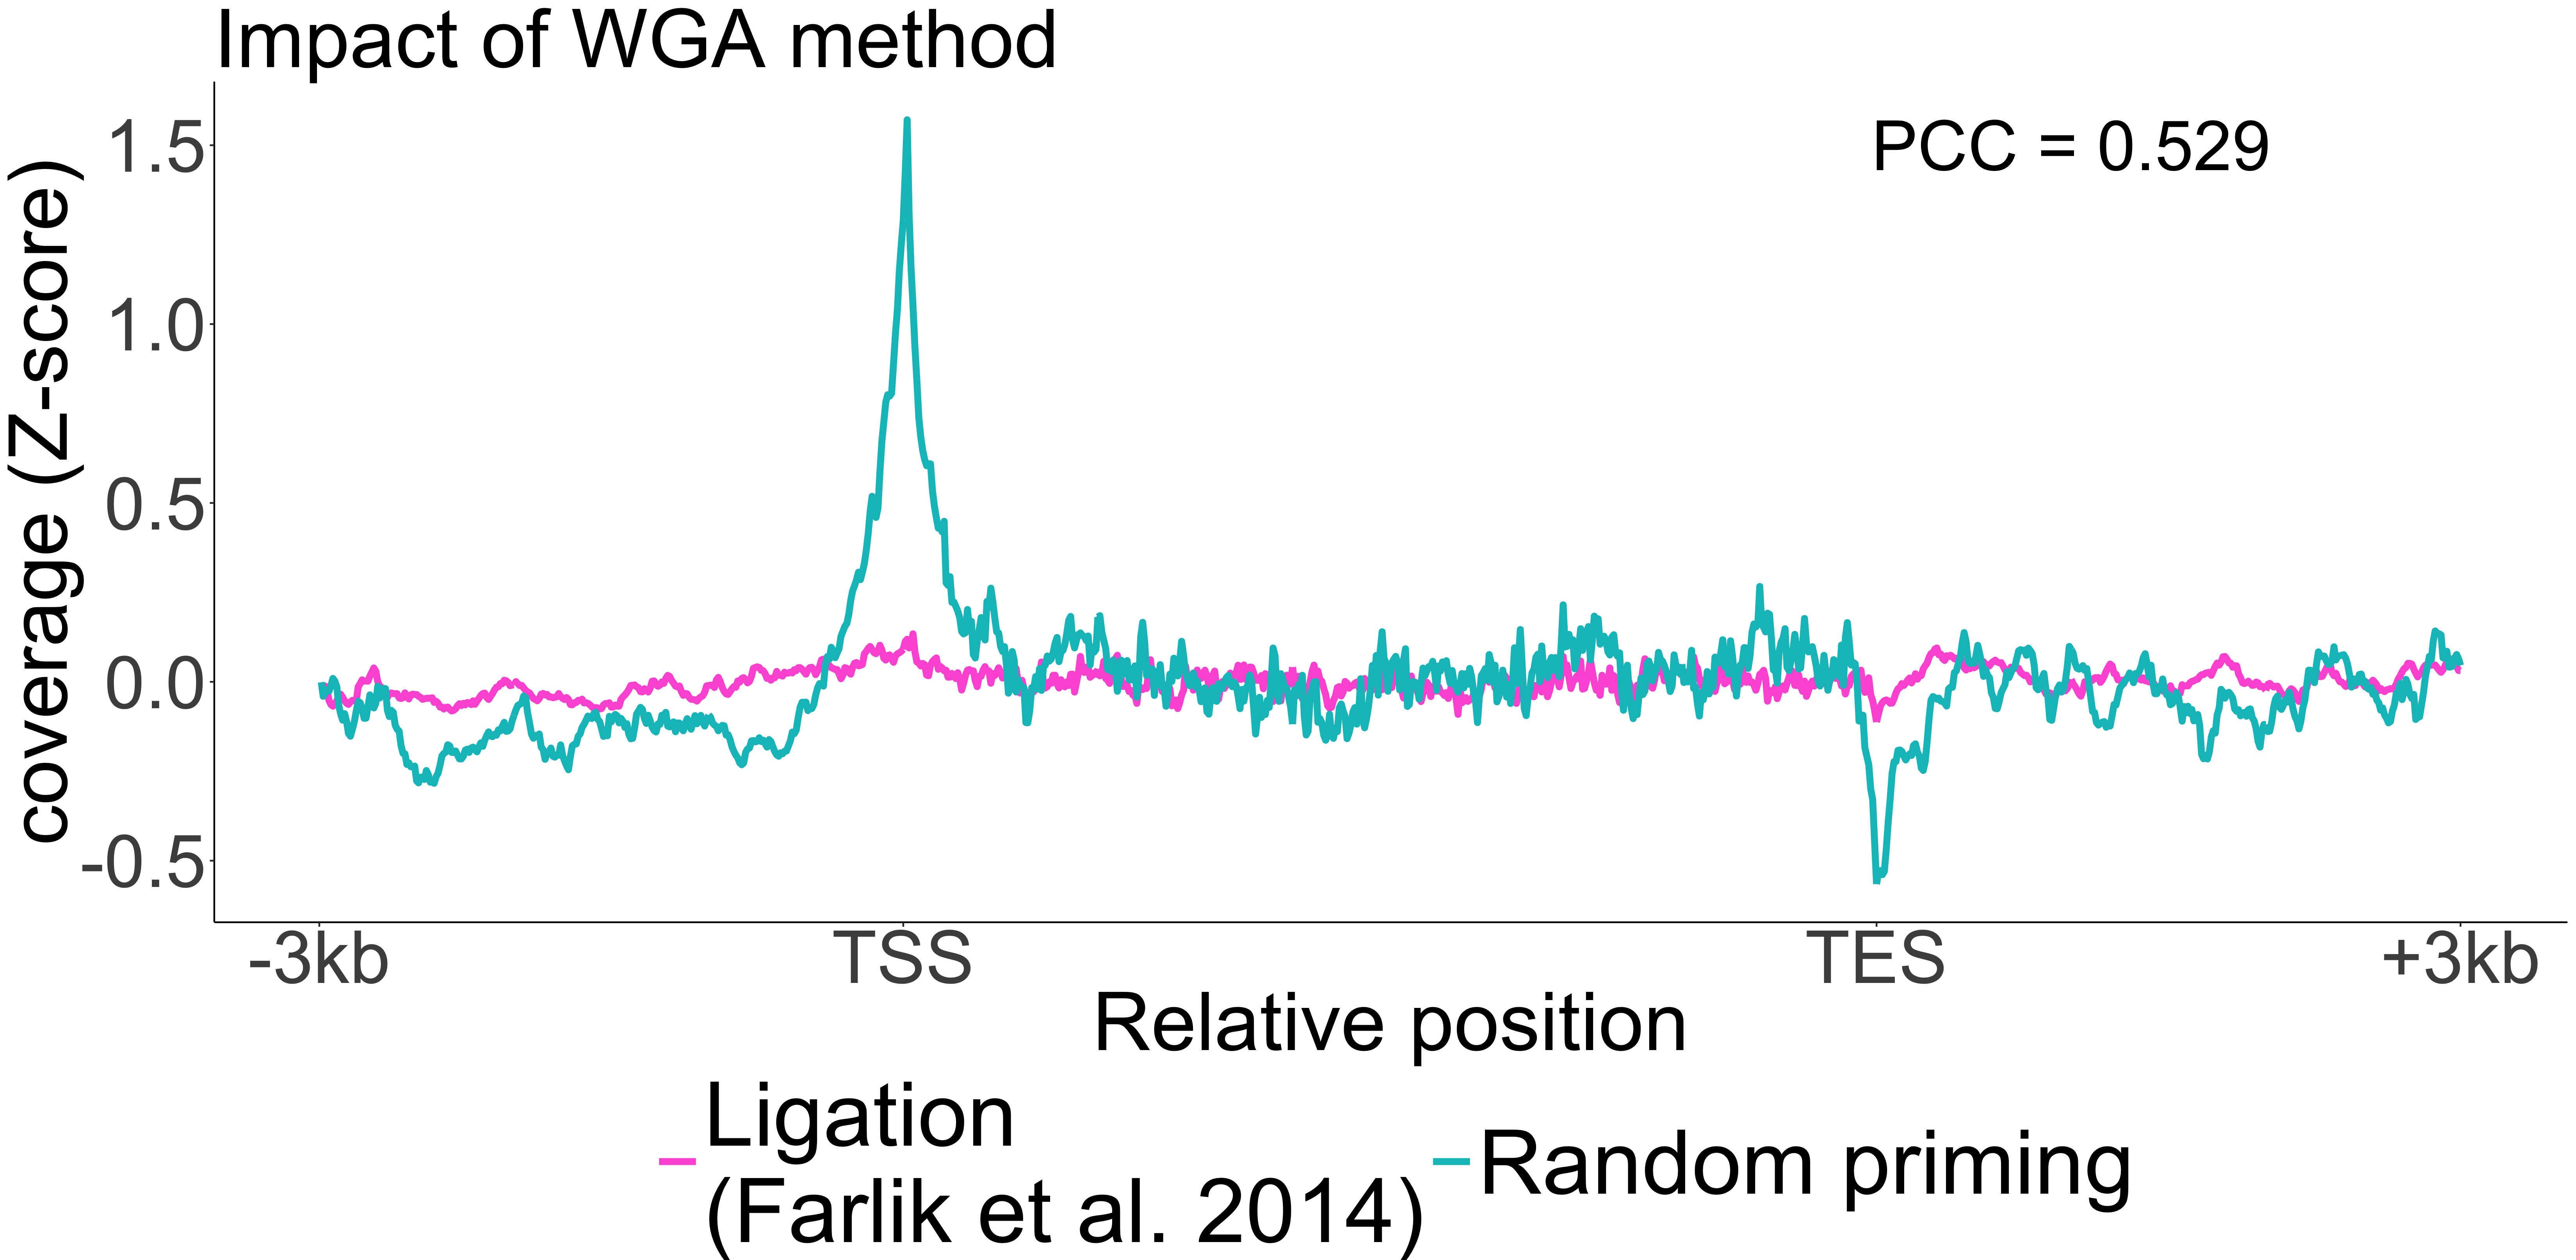
\includegraphics[scale = 0.03]{wga_bias.png}
  \end{figure}
\end{frame}

\begin{frame}[label=current]{Modelling random hexamer binding}
  \vspace{-2cm}
  \begin{figure}
      \centering
      
\includegraphics[scale=0.25, trim={0 3cm 0 8cm}, clip]{template_primer.png}
  \end{figure}
\begin{figure}
  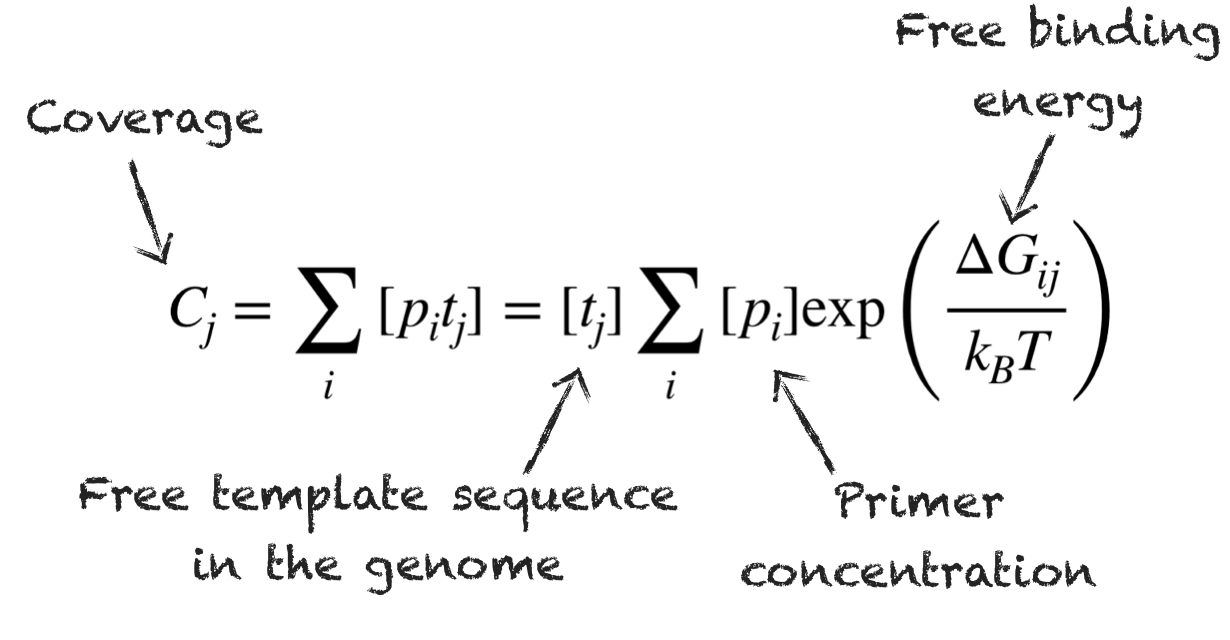
\includegraphics[scale=0.3]{model_w_labels.png}
\end{figure}
\begin{itemize}
  \item High frequency of mismatching primer-template events
  \item Lack of tabulated $\Delta$G values for non Watson-Crick base pairing
  \item Difficult to determine exact genomic kmer abundance for BS converted genome
\end{itemize}
\end{frame}
%
% \begin{frame}{Modelling random hexamer binding}
%   \begin{equation*}\label{eq: DeltaG}
%   \frac{[pt]}{[t]} = [p]\exp\left(\beta\Delta G\right).
%   \end{equation*}
%   \begin{figure}
%       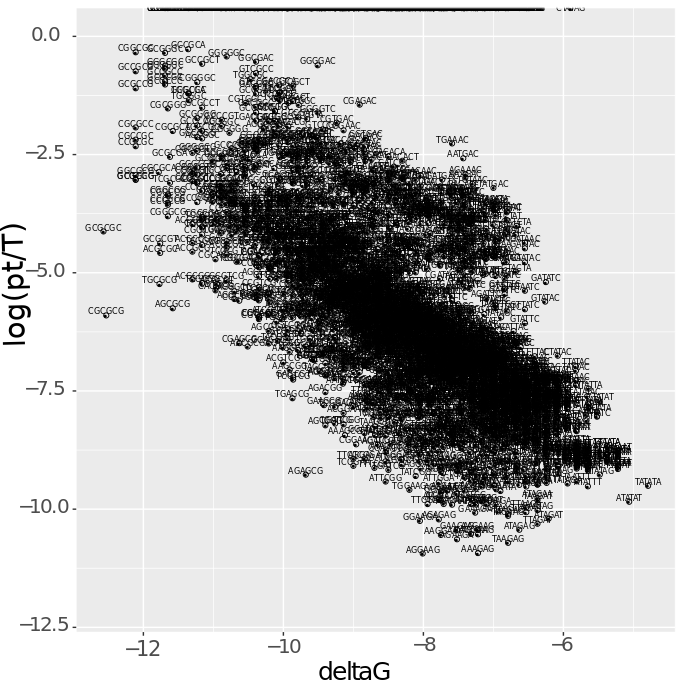
\includegraphics[scale=0.25]{occupancy_ab_amp_bigLabels.png}
%   \end{figure}
% \end{frame}
%
% \begin{frame}{Frequent mismatches at primer binding position in BS seq data}
%   \Wider{
%   \begin{columns}
%   \begin{column}{0.5\linewidth}
%       \begin{figure}
%           \centering
%           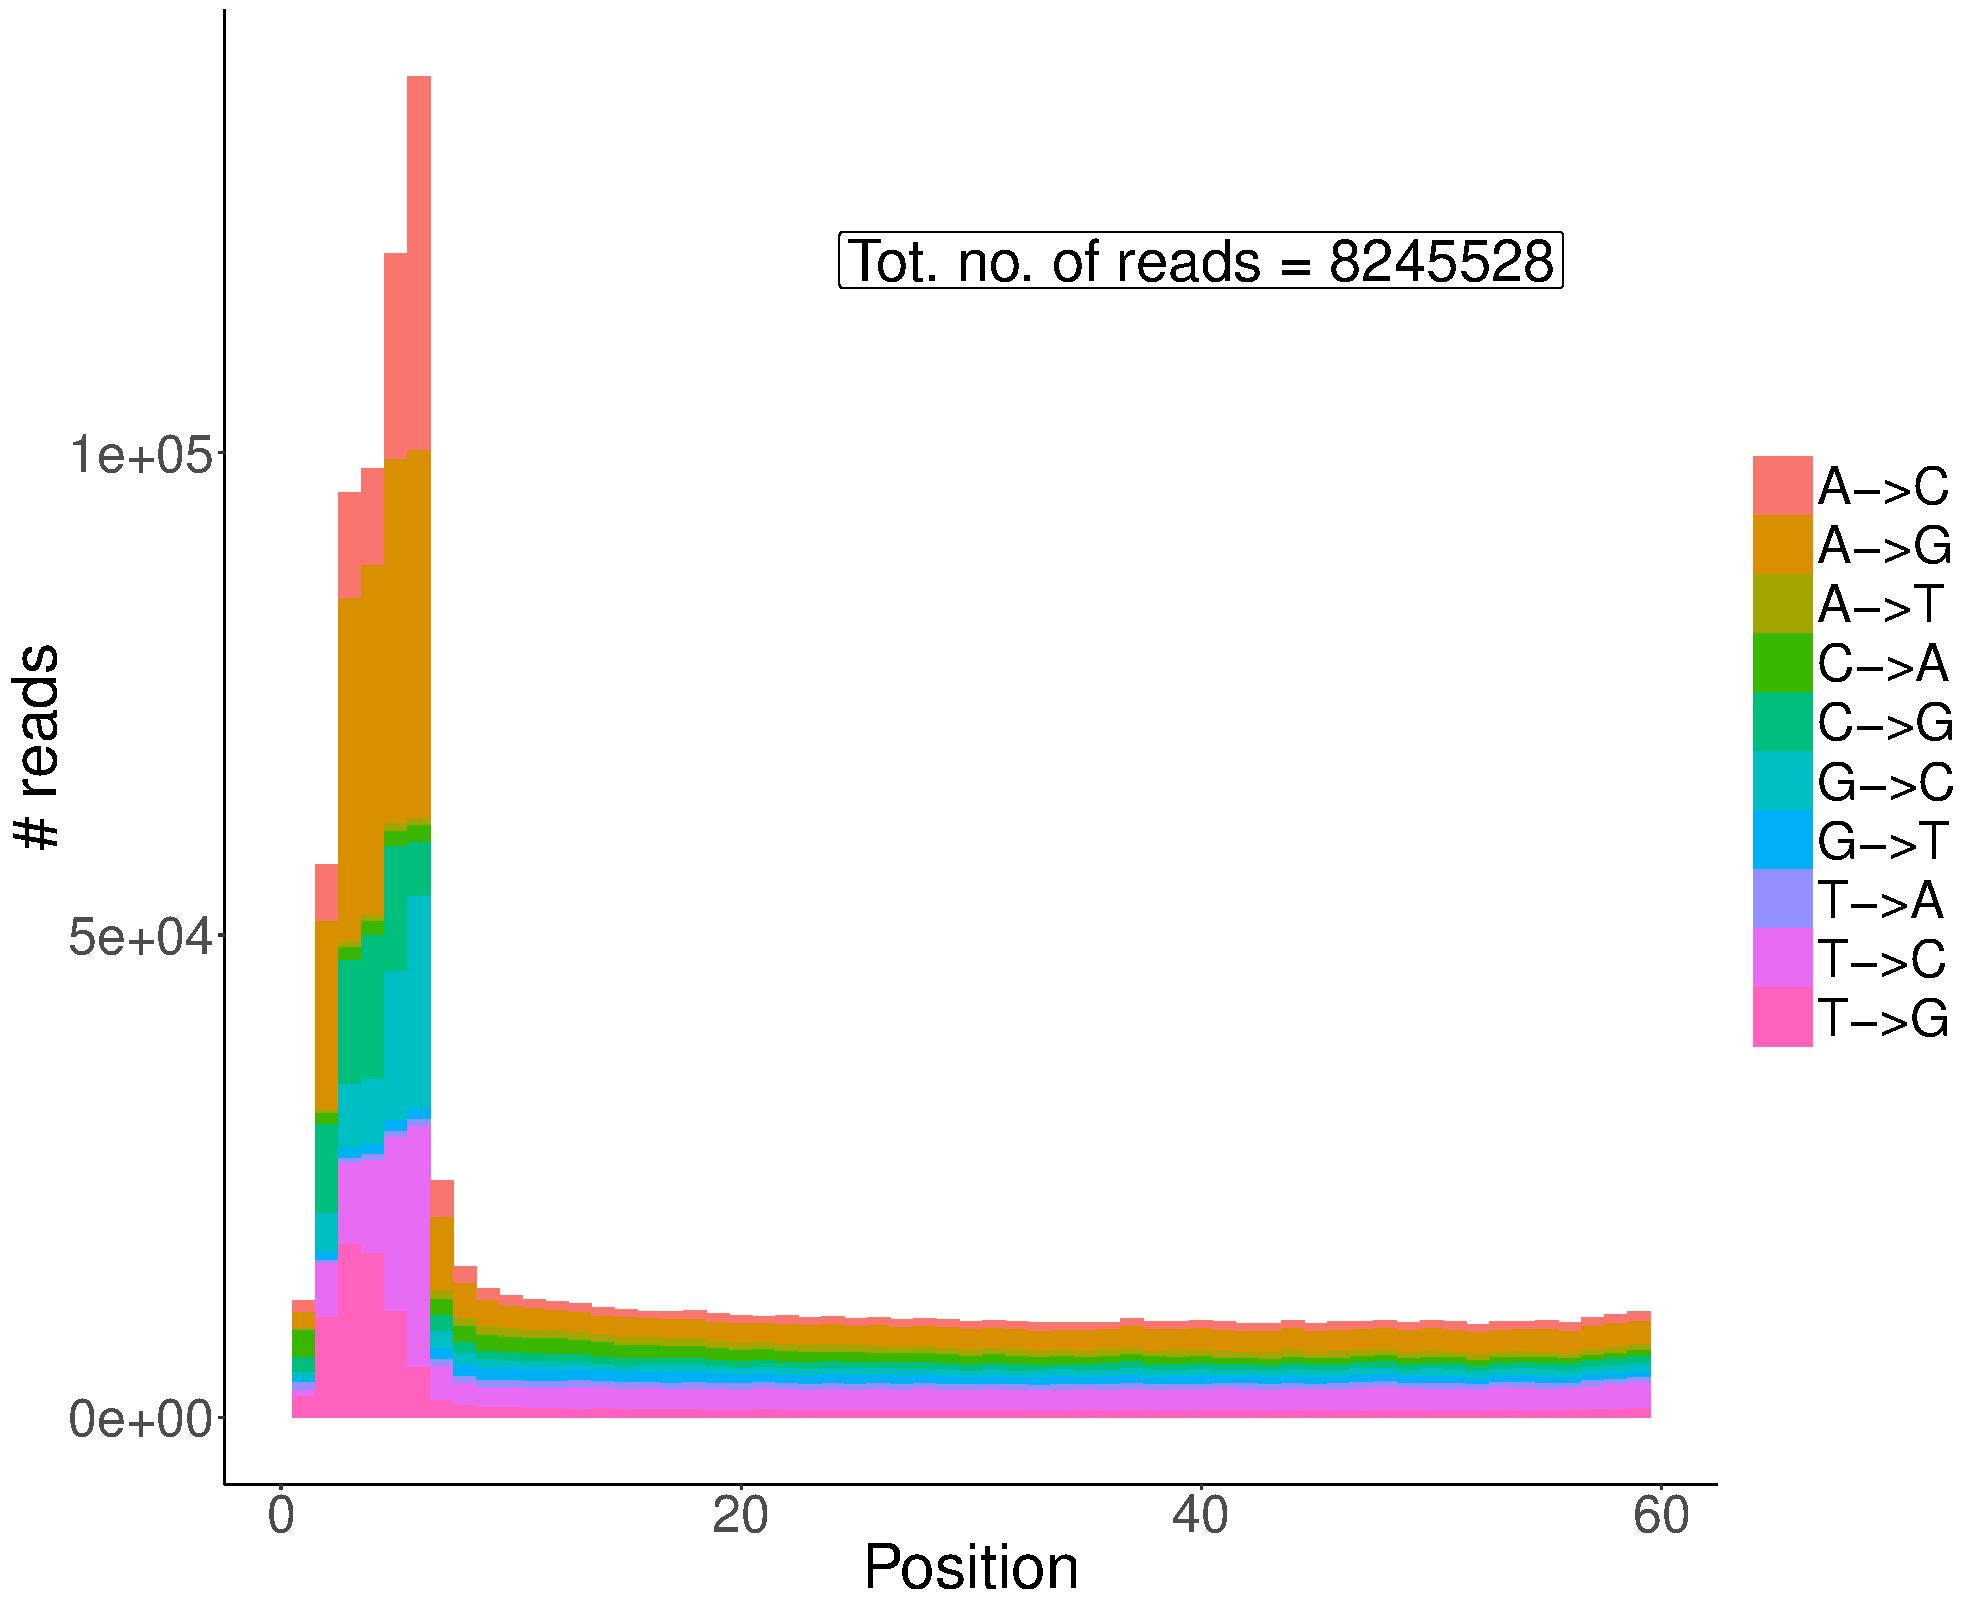
\includegraphics[scale=0.2]{mismatch_per_position_abs_L1.pdf}
%       \end{figure}
%   \end{column}
%   \begin{column}{0.45\linewidth}
%   \begin{figure}
%       \centering
%       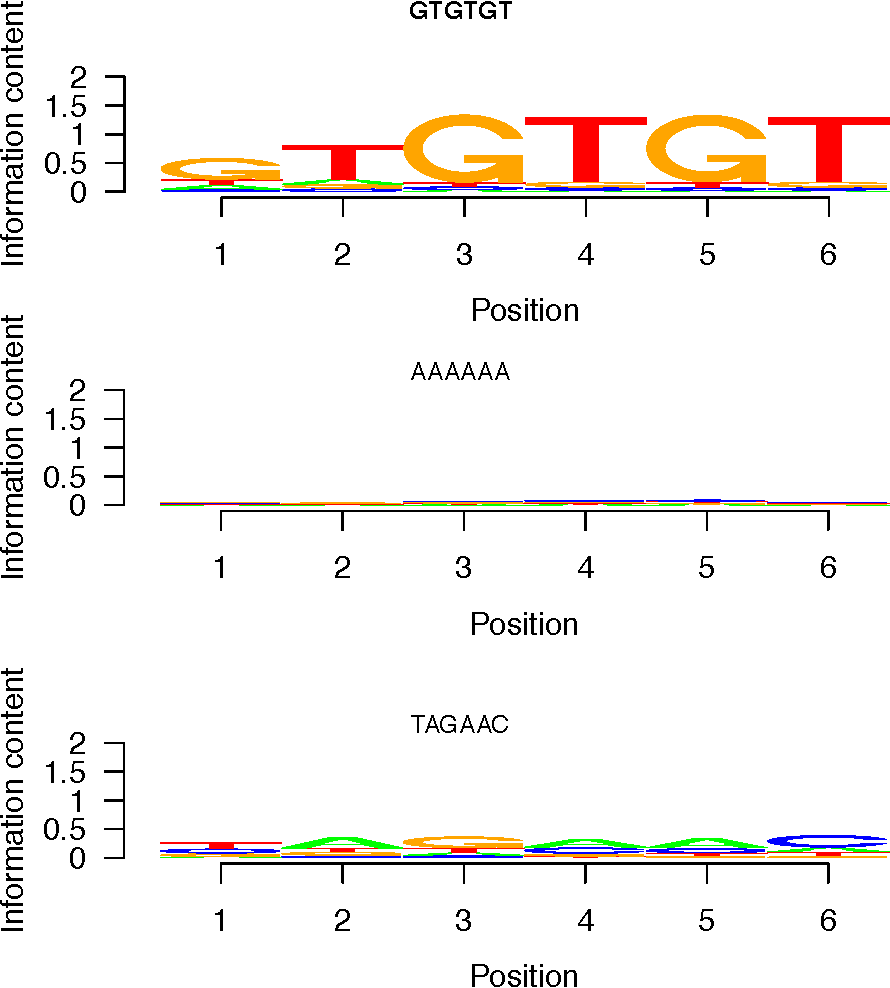
\includegraphics[scale=0.3, trim={0 5cm 0 0}, clip]{seqLogos_templ_ordBindingEvTempl.pdf}
%   \end{figure}
%   \end{column}
%   \end{columns}
%   }
% \end{frame}
%
% \begin{frame}{Hexamer binding model 2.0: accounting for all binding events}
%   \vspace{-0.4cm}
%   \begin{figure}
%       \centering
%       
\includegraphics[scale=0.3]{template_primer.png}
%   \end{figure}
%   \begin{equation*}
%   p_i+t_j \rightleftarrows p_it_j,
%   \end{equation*}
%   where $p_it_j$ is the binding complex. In equilibrium conditions it is satisfied that:
%   \begin{equation*}
%   \frac{[p_it_j]}{[p_i][t_j]} = \exp\left(\beta\Delta G_{ij}\right).
%   \end{equation*}
%
%   \onslide<2-3>{
%   How to define coverage?
%   \begin{equation*}
%   C_j = \sum_i[p_it_j] = \boxed{T_j\frac{\sum_i[p_i]\exp\left(\beta\Delta G_{ij}\right)
%   }{\left[1+\sum_i[p_i]\exp\left(\beta\Delta G_{ij}\right)\right]}}
%   \end{equation*}
%
%   $T_j = t_j + C_j$ $\longrightarrow$ total abundance of template sequence ; \\ $[p_i]$ $\longrightarrow$ concentration of primers in the experiments. \\
%   }
%   \onslide<3>{
%   \begin{center}
%     \alert{\large{What about $\Delta G_{ij}$ ?}}
%   \end{center}
%   }
% \end{frame}
%
%
% \begin{frame}{Computing $\Delta G_{ij}$ from sequencing data}
%   \Wider{
%   \begin{equation*}
%   \frac{[p_it_j]}{[p_i][t_j]} = \exp\left(\beta\Delta G_{ij}\right).
%   \end{equation*}
%   \begin{figure}
%       \only<1>{\includegraphics[scale=0.47,page=12, trim={0 2cm 0 2cm}, clip]{counting-3.pdf}}
%       \only<2>{\includegraphics[scale=0.47,page=13, trim={0 2cm 0 2cm}, clip]{counting-3.pdf}}
%       \only<3-4>{\includegraphics[scale=0.47,page=14, trim={0 2cm 0 2cm}, clip]{counting-3.pdf}}
%   \end{figure}
%   \onslide<4>{
%     \centering{\alert{\large{How to use this approach on bisulfite converted genome?}}}}
%     }
% \end{frame}
%
%
% \begin{frame}{Prediction on BS-seq data}
%   \vspace{-0.5cm}
%   \begin{figure}
%       \centering
%       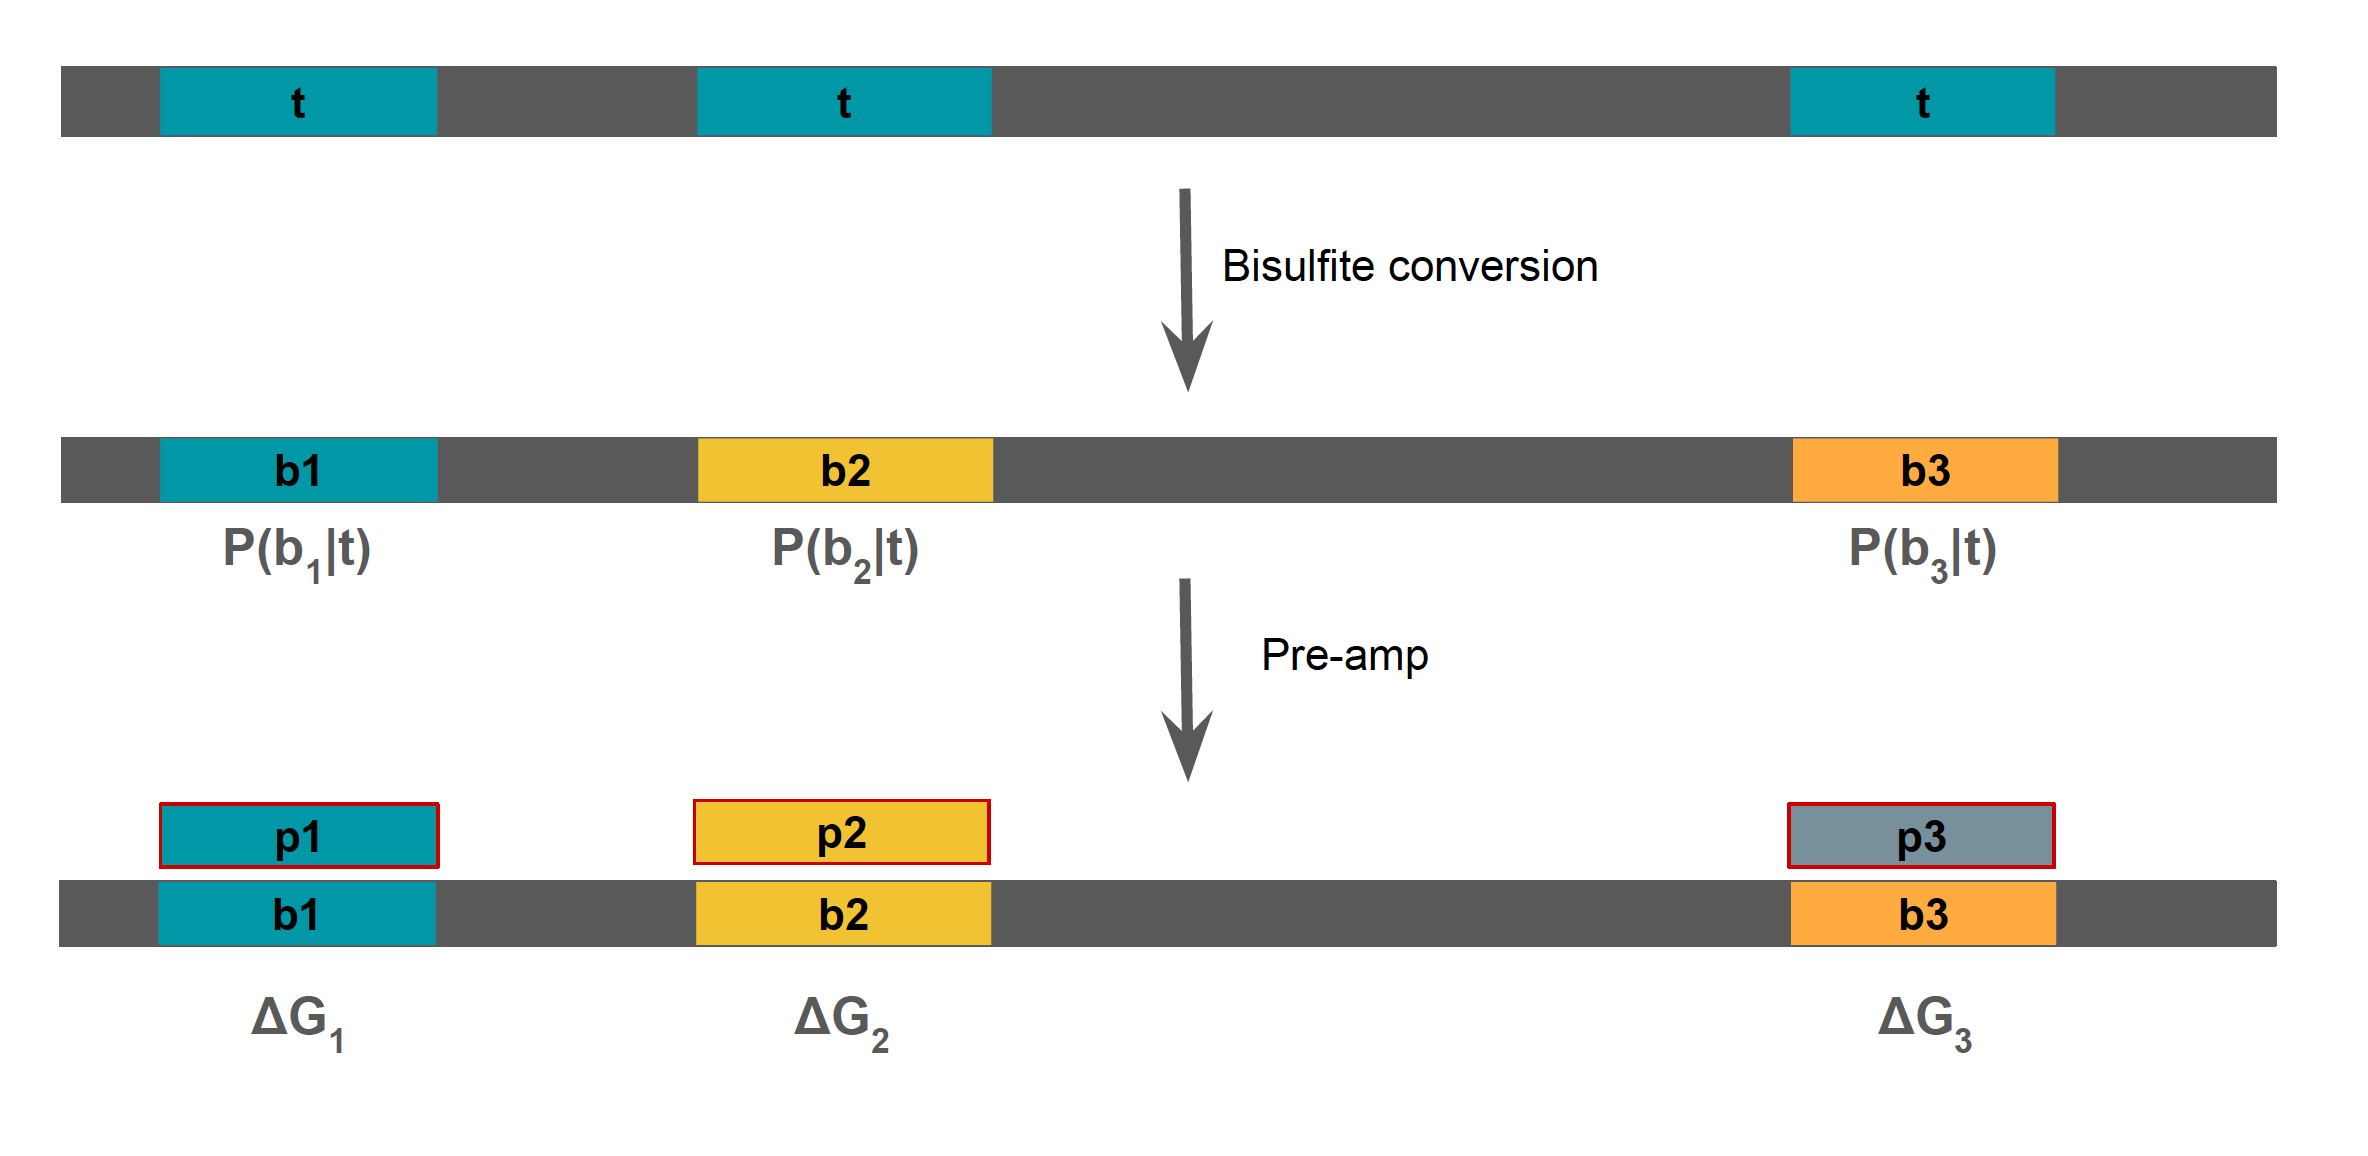
\includegraphics[scale=0.2]{bs_model.png}
%   \end{figure}
%   \begin{equation*}
%   \begin{split}
%        [p_i t] & = [b_1 p_i] + [b_2 p_i] + [b_3 p_i] ... \\
%               %  & = [t]P(b_1|t)[p]\sum_i \exp\left(\frac{\Delta G_{1i}}{k_BT}\right) + [t]P(b_2|t)[p]\sum_i \exp\left(\frac{\Delta G_{2i}}{k_BT}\right) + [t]P(b_3|t)[p]\sum_i \exp\left(\frac{\Delta G_{3i}}{k_BT}\right) \\
%                \onslide<2-4>{ & =[b_1][p_i]\exp\left(\beta\Delta G\right) + [b_2][p_i]\exp\left(\beta\Delta G\right) + ... \\}
%                \onslide<3-4>{ & =[t][p_i]\sum_n \exp\left(\beta\Delta G\right) P(b_n|t) \\}
%                \onslide<4>{ & =[t][p_i] \exp\left(\beta\Delta F\right) \\}
%   \end{split}
%   \end{equation*}
% \end{frame}
%
% \begin{frame}{Validating $\Delta$F: consistency between experiments}
%   \vspace{-0.2cm}
%   \begin{figure}
%       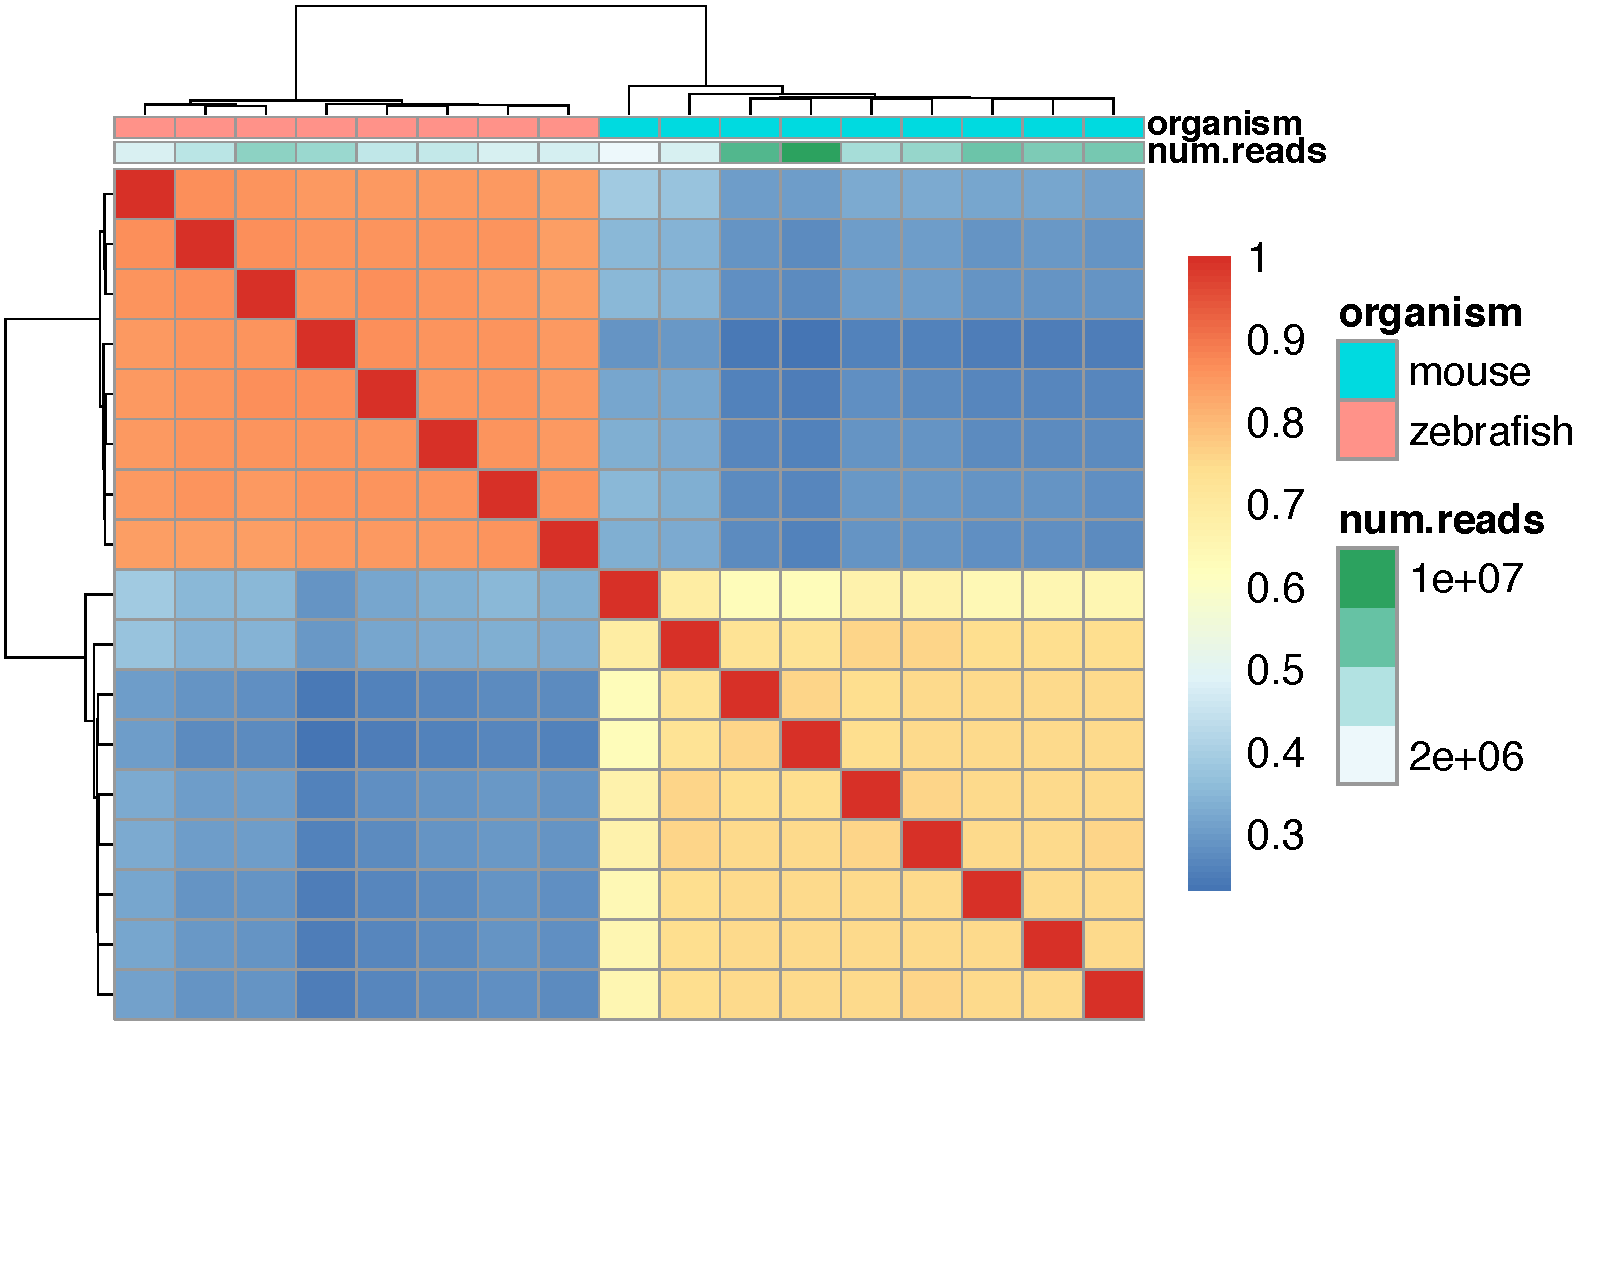
\includegraphics[scale=0.35]{BScorrelation_deltaG_R1.pdf}
%   \end{figure}
% \end{frame}
%
% \begin{frame}{Validating $\Delta$F: consistency with tabulated free-binding energy values}
%   \vspace{-0.3cm}
%       \centering{Hexamers with no C $\longrightarrow \Delta F \equiv \Delta G$}
%       \begin{figure}
%           \centering
%           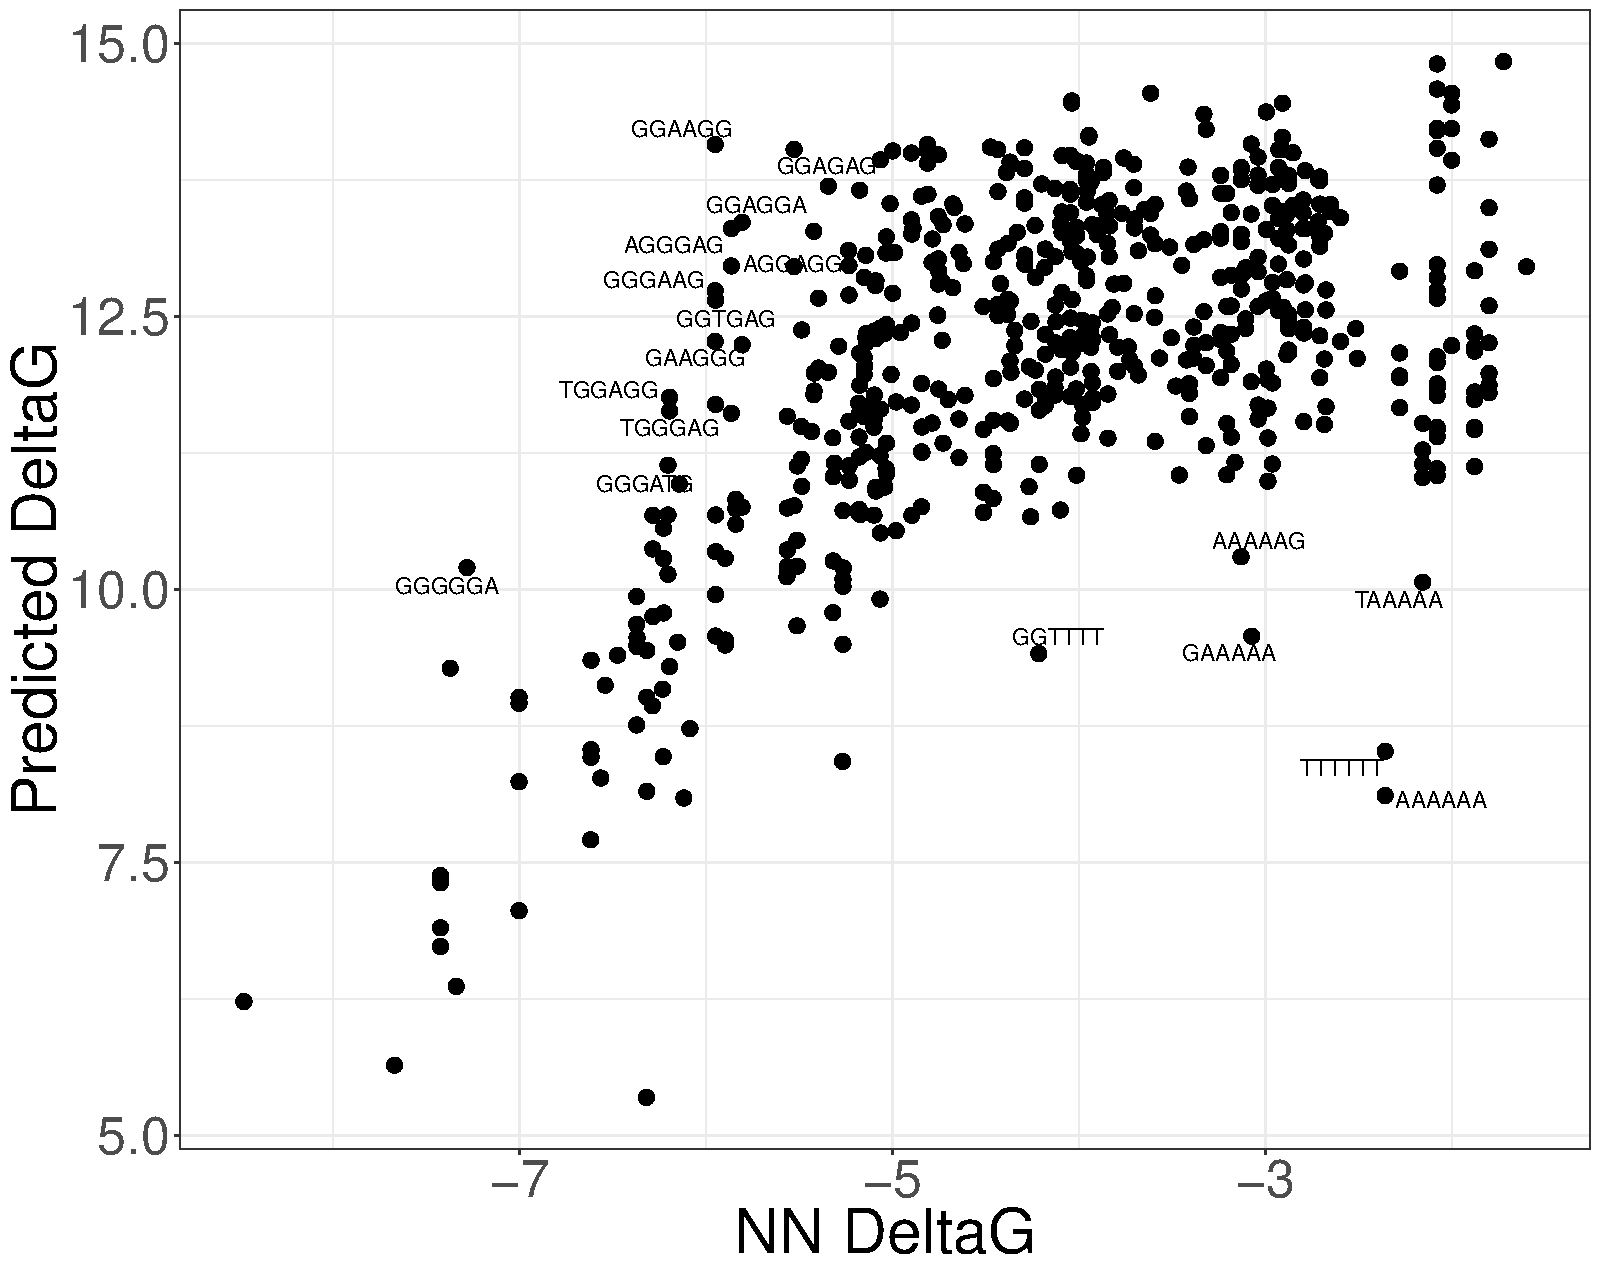
\includegraphics[scale=0.27]{predBsVSnnmodel_noC_strandSpecific.pdf}
%       \end{figure}
%   \onslide<2>{
%   \begin{center}
%     \alert{Ongoing: generating data on non-converted samples for \\
%     validation of $\Delta G$ prediction}
%   \end{center}
%   }
% \end{frame}
%
% \begin{frame}{Predicted coverage from $\Delta$F}
%   \begin{figure}
%       \centering
%       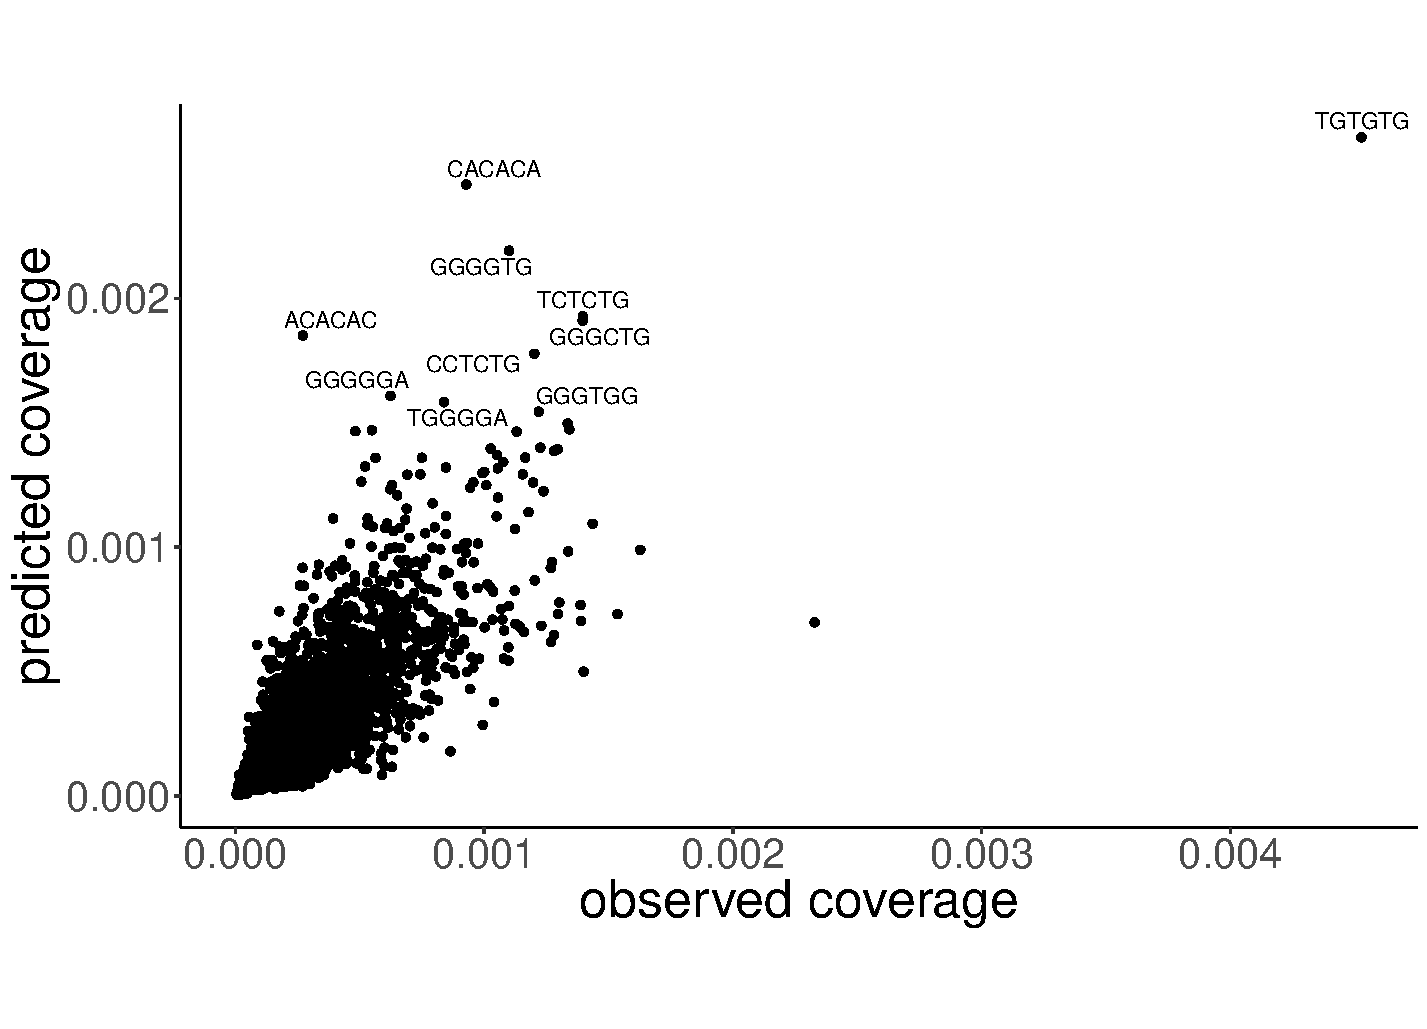
\includegraphics[scale=0.35]{predictedCov_VAN1815_L2_pooledVAN1667.pdf}
%       % \caption{Caption}
%       % % \label{fig:my_label}
%   \end{figure}
%   \onslide<2>{
%   \begin{center}
%     \alert{Does binding explain the spatial genome-wide distribution of coverage?}
%   \end{center}
%   }
% \end{frame}
%
% \begin{frame}{Positional information from binding probability}
%   \Wider{
%   \vspace{-0.4cm}
%   % \centering{Coverage density: $D_j = \frac{C_j}{T_j}$}
%   \begin{figure}
%     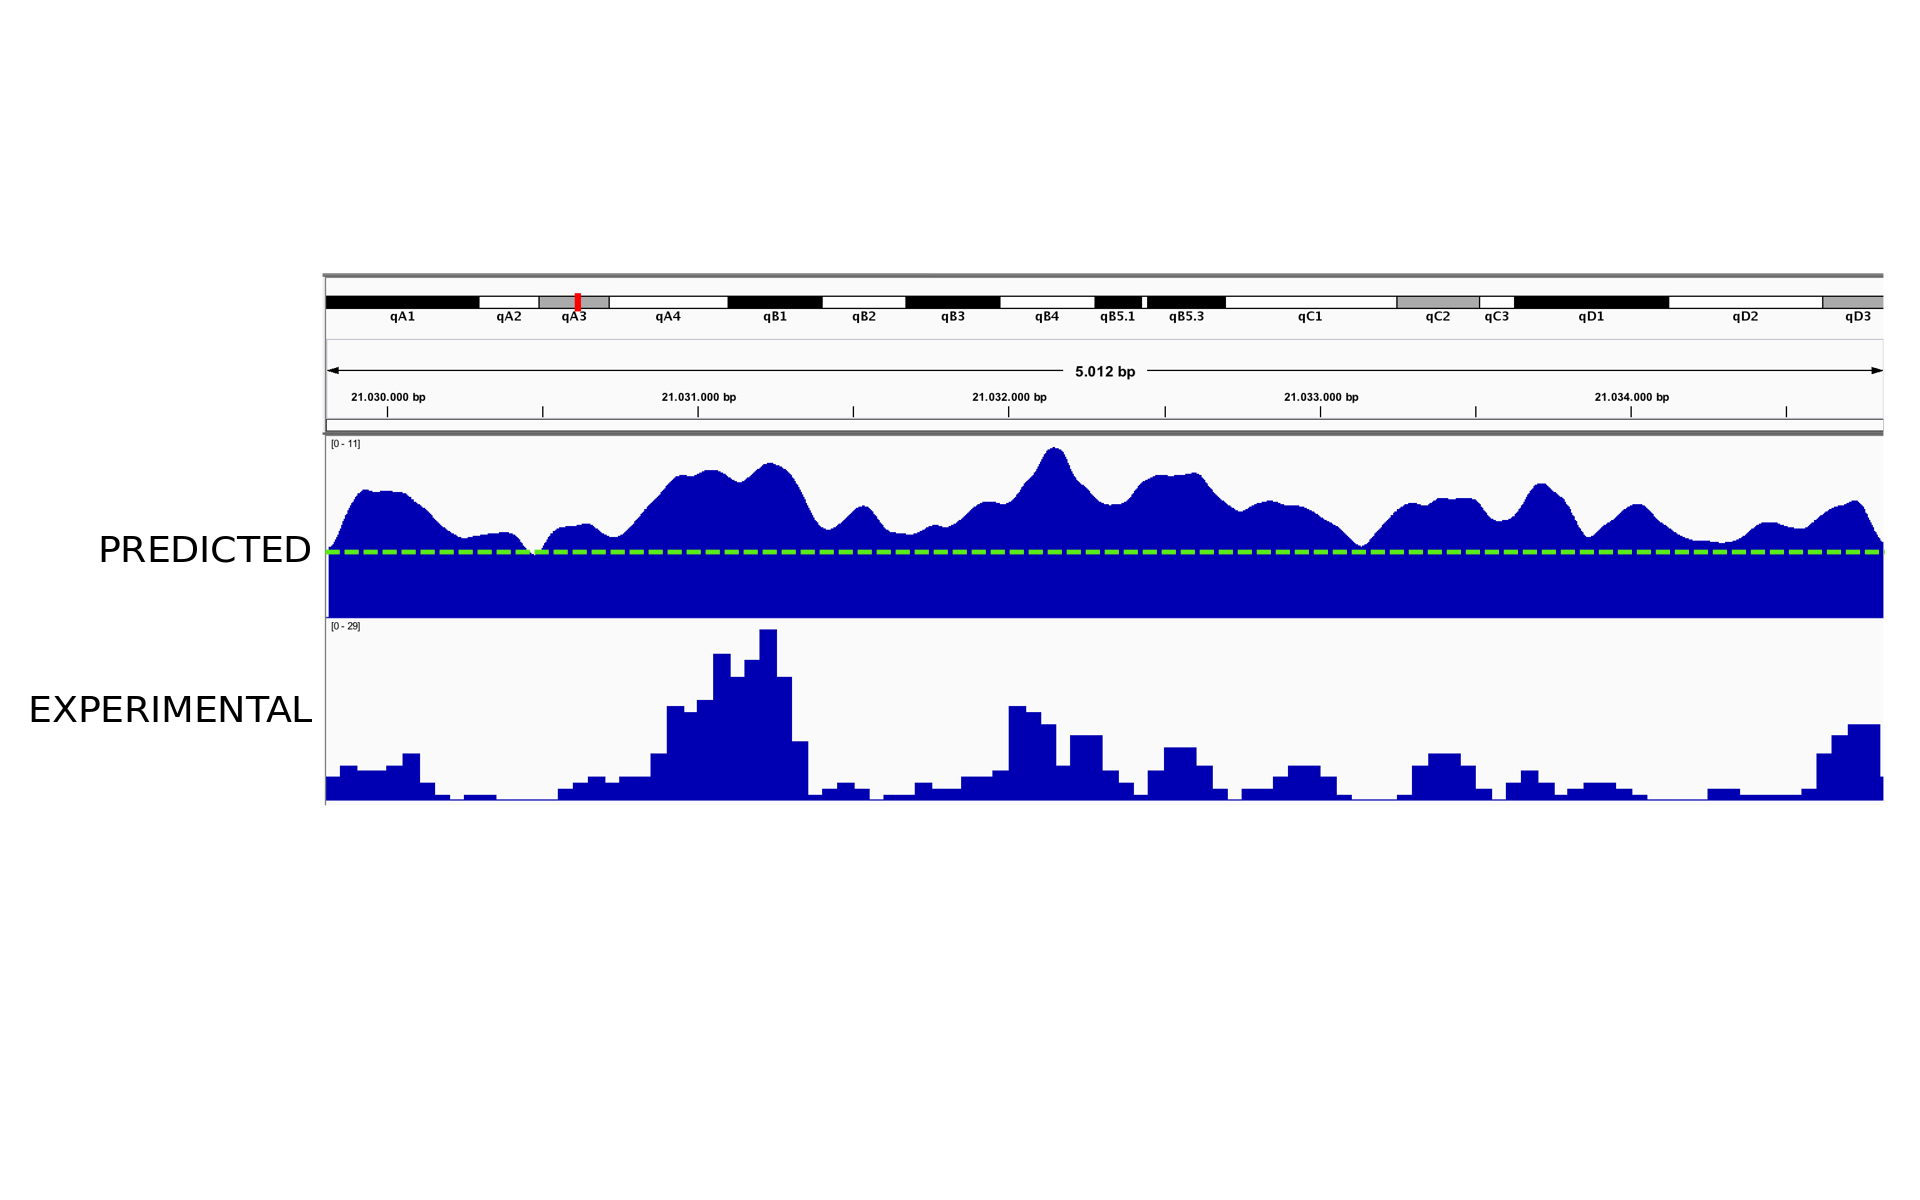
\includegraphics[scale=0.15, trim={0 14cm 0 9cm}, clip]{strand_specific_artcov.png}
%   \end{figure}
%   \onslide<2>{
%   \vspace{-0.4cm}
%   \begin{figure}
%     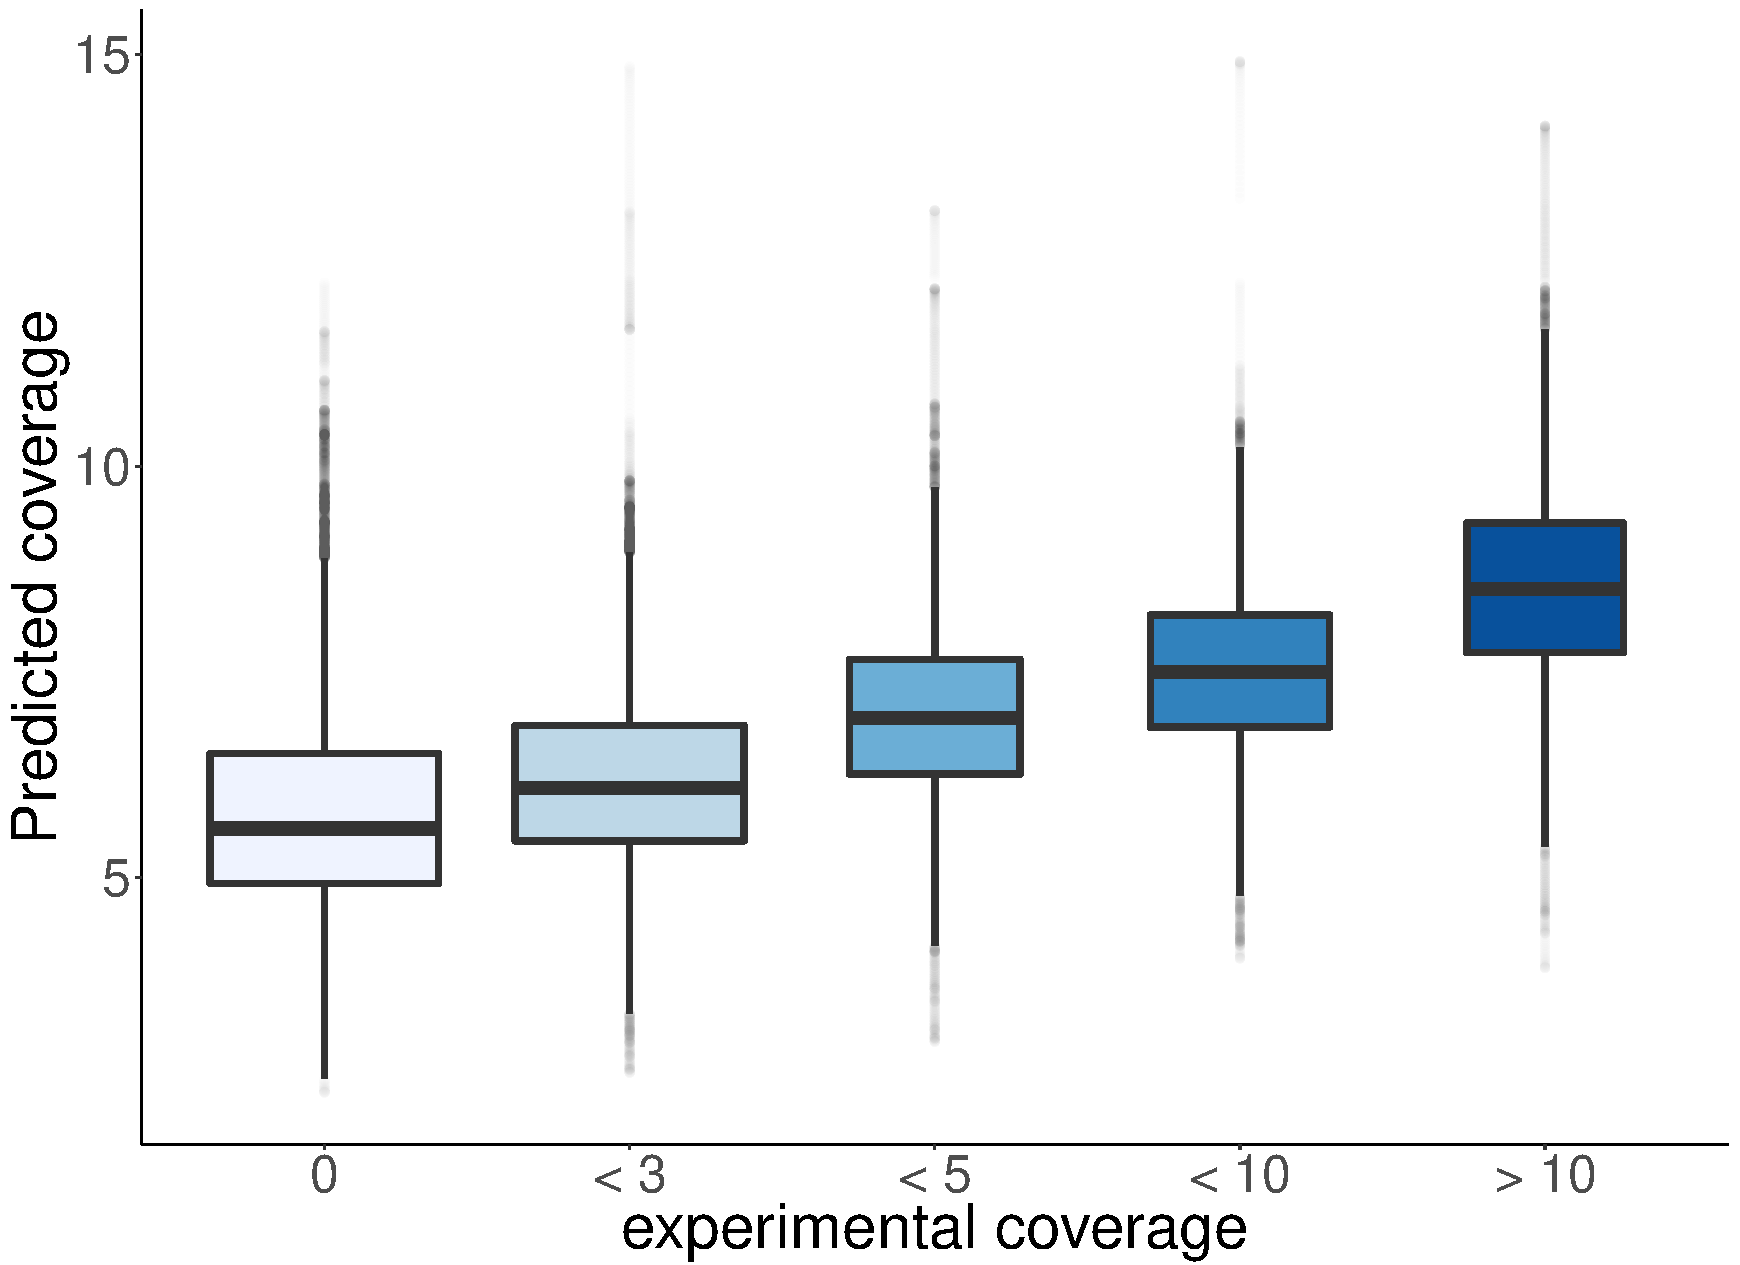
\includegraphics[scale=0.2]{predVSexperimental_boxplot.pdf}
%   \end{figure}
%   }
%   }
% \end{frame}
%
% % \begin{frame}{How much of the bias can be explained by binding events?}
% %   \begin{figure}
% %     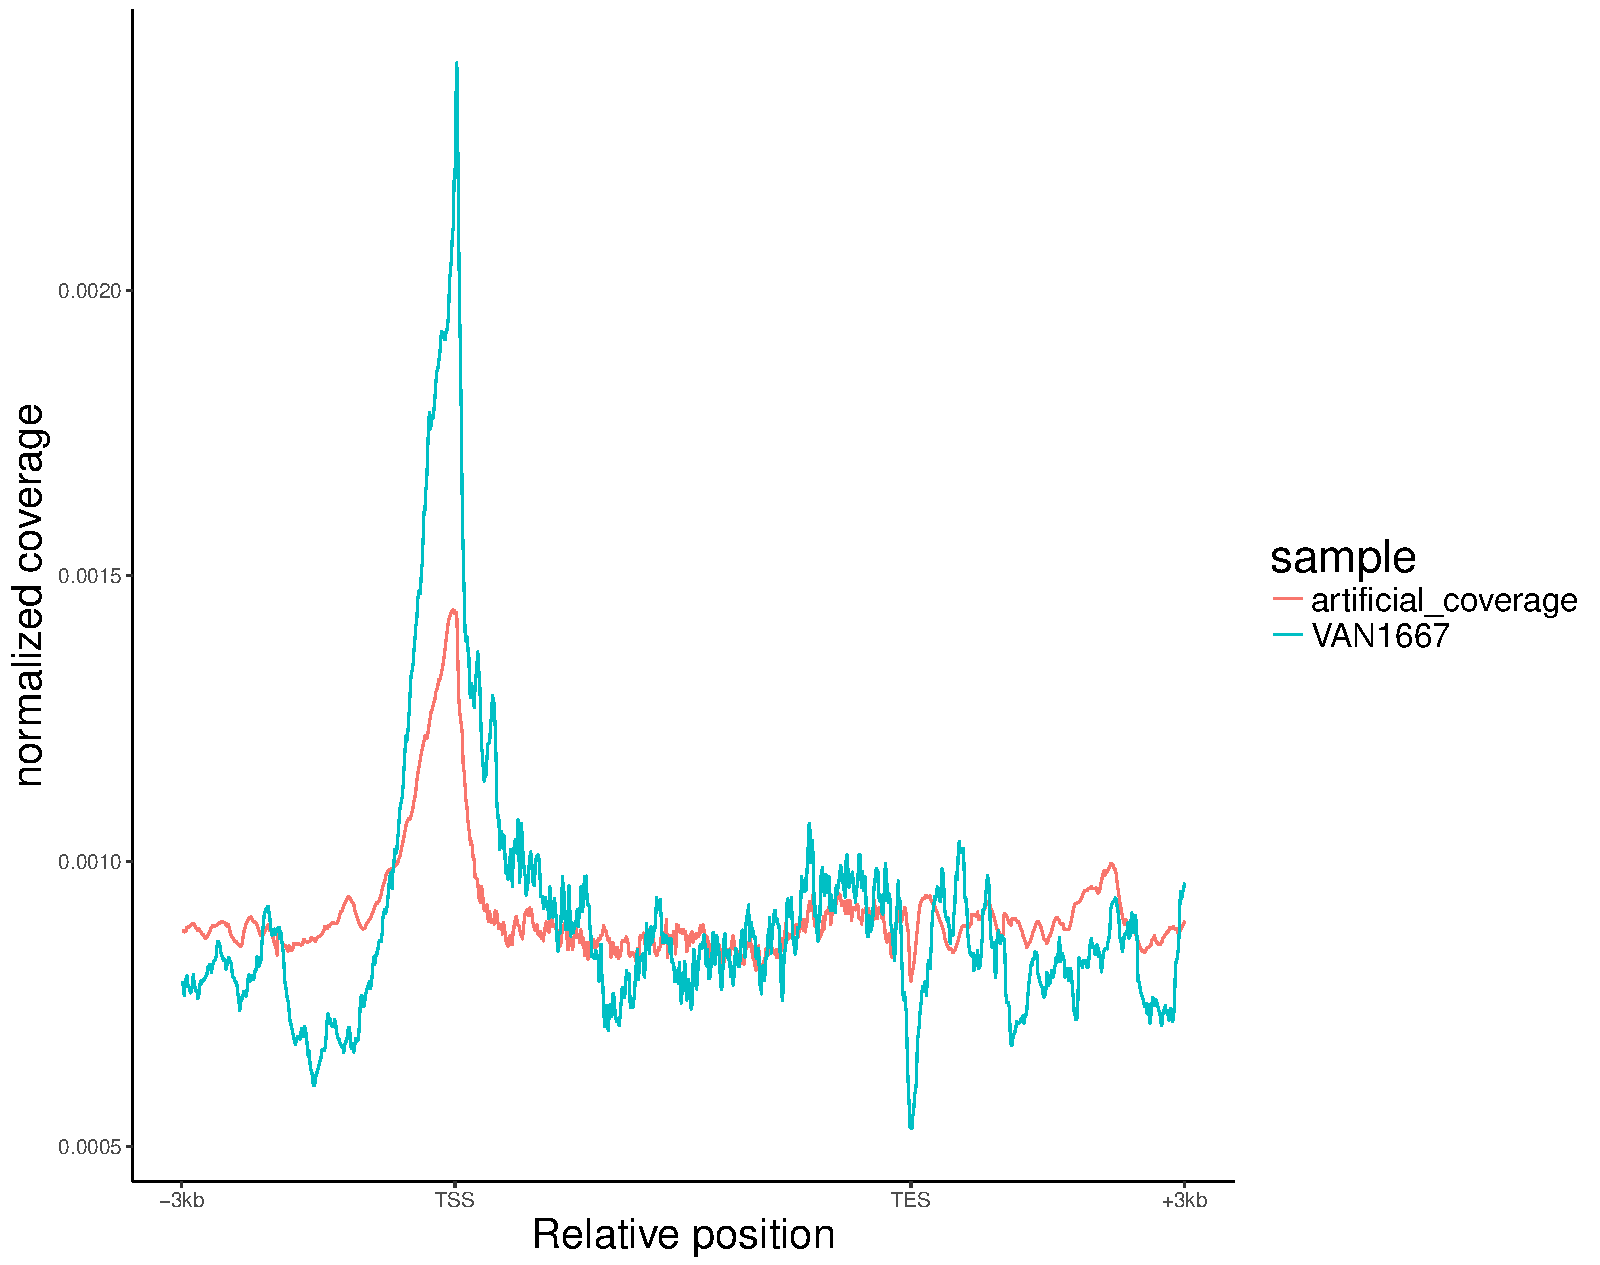
\includegraphics[scale=0.3]{bias_artCovVSVAN1667subsmp.pdf}
% %   \end{figure}
% % \end{frame}
%
% \begin{frame}{Next steps: optimizing the primer pool}
%   \begin{columns}
%   \begin{column}{0.5\linewidth}
%     \begin{itemize}
%       \item Altering the coverage by changing primer concentration
%       \item Finding the optimal primer composition matrix (Differential evolution algorithm)
%     \end{itemize}
%   \end{column}
%   \begin{column}{0.5\linewidth}
%     \animategraphics[scale=0.3, autoplay]{7}{DE_iter-}{1}{99}
%     % \includegraphics{test_iter-1.png}
%   \end{column}
%   \end{columns}
% \end{frame}
%
% \appendix
%
% \begin{frame}{Acknowledgements}
%   \begin{columns}
%     \begin{column}{0.4\linewidth}
%       \begin{itemize}
%         \item \textbf{Alexander Van Oudenaarden}
%         \item \textbf{Christoph Geisenberger}
%         \item \textbf{Anna Alemany Arias}
%         \item Juan Pedraza
%         \item Anna Van Oudenaarden
%         \item Maya Sen
%         \item Lennart Kaester
%         \item Buys de Barbanson
%         \item the AvO lab
%       \end{itemize}
%     \end{column}
%     \begin{column}{0.6\linewidth}
%       \begin{figure}
%         
\includegraphics[scale=0.3, trim={0 3cm 3.5cm 0}, clip]{image002.png}
%       \end{figure}
%     \end{column}
%   \end{columns}
% \end{frame}

% \begin{frame}{Ruling out other sources of bias}
% Accessibility
% Primer concentration
% \end{frame}

\end{document}
